\documentclass[12pt]{article}

\usepackage[a4paper,margin=1in]{geometry}
\usepackage{amsmath,amssymb,amsfonts}
\usepackage{graphicx}
\usepackage{booktabs}
\usepackage{float}
\usepackage{hyperref}
\usepackage{setspace}
\usepackage{caption}
\usepackage{cite} % لإدارة المراجع

\hypersetup{
    colorlinks=true,
    linkcolor=black,
    citecolor=black,
    urlcolor=blue
}

\captionsetup{font=small}
\setstretch{1.15}

% ==========================================================
% عنوان الصفحة (متطلبات النشر: صفحة عنوان منفصلة)
% ==========================================================
\title{\textbf{A Hybrid Quantum--Classical Optimization Framework for Well Placement in Oil Reservoirs Using QUBO Modeling and QAOA}}

\author{
Tareq Mageed$^{1,\ast}$ \\[0.5em]
$^{1}$Ministry of Oil, Iraq \\ 
Dhi Qar Oil Company \\
Quality Management and Institutional Development Division \\[0.5em]
$\ast$Corresponding author: \href{mailto:tariq.mageed@gmail.com}{tariq.mageed@gmail.com}
}

\date{}

\begin{document}

\maketitle

\begin{abstract}
Optimal well placement is a central decision problem in field development planning because it directly affects production performance and project economics. The combinatorial nature of the problem makes exhaustive search infeasible for large candidate sets. This study presents a hybrid quantum--classical optimization framework for well placement using Quadratic Unconstrained Binary Optimization (QUBO) modeling and the Quantum Approximate Optimization Algorithm (QAOA). The framework reformulates well selection as a binary optimization problem with production rewards and distance-dependent interference penalties. A controlled four-well validation benchmark is used, allowing exact comparison against brute-force enumeration and simulated annealing.

The implementation demonstrates that the QAOA-based solution recovers the global optimum exactly, achieving an approximation ratio of 1.0. The results confirm the mathematical correctness of the QUBO formulation and the algorithmic validity of the QAOA implementation on a fully verifiable benchmark. Supporting visualizations are generated to compare energy, production, interference, and runtime across methods.
\end{abstract}

\section{Introduction}

Well placement optimization is a combinatorial problem where the objective is to select a subset of candidate wells that maximizes production while minimizing interference. For \(N\) candidate wells, the search space consists of \(2^{N}\) configurations. Classical metaheuristics such as simulated annealing are widely used, but quantum-inspired methods offer an alternative approach that can be systematically benchmarked.

The Quantum Approximate Optimization Algorithm (QAOA) is a variational algorithm designed for problems expressible in Ising or QUBO form \cite{farhi2014quantum}. In this work, the well placement problem is cast as a QUBO model, and a depth-\(p = 2\) QAOA circuit is executed on a classical simulator. The results are compared against brute-force enumeration and simulated annealing. The validation benchmark consists of \(N = 4\) wells, which allows complete enumeration of \(2^{4} = 16\) configurations and provides a rigorous correctness check.

\section{Problem Formulation}

Let \(x_{i} \in \{0,1\}\) be the binary decision variable for well \(i\), where \(x_{i} = 1\) indicates selection. The objective energy is defined as:
\begin{equation}
E(x) = x^{T}Qx 
\label{eq:qubo_energy}
\end{equation}
where \(Q \in \mathbb{R}^{N \times N}\) is the QUBO matrix.

\section{QUBO Construction}

The diagonal terms of \(Q\) encode production rewards:
\begin{equation}
Q_{ii} = -P_{i} 
\label{eq:diagonal}
\end{equation}
where \(P_{i}\) is the production potential of well \(i\). In the validation benchmark, the production potentials are:
\begin{equation}
P = [0.9, \; 0.3, \; 0.8, \; 0.2]
\label{eq:production_values}
\end{equation}

The off-diagonal terms represent spatial interference between wells \(i\) and \(j\):
\begin{equation}
Q_{ij} = 0.2 \exp\left(-\frac{d_{ij}}{\lambda}\right), \quad i \neq j
\label{eq:interference}
\end{equation}
where \(d_{ij}\) is the Euclidean distance between well coordinates, and \(\lambda = 400.0\) is the decay length. The well coordinates used in the benchmark are:
\begin{align*}
\text{Well 0:} & \quad (0.0, 0.0) \\
\text{Well 1:} & \quad (500.0, 0.0) \\
\text{Well 2:} & \quad (0.0, 500.0) \\
\text{Well 3:} & \quad (500.0, 500.0)
\end{align*}

This formulation creates a natural trade-off: selecting high-production wells is favored, but closely spaced wells incur an interference penalty.

\section{Optimization Methods}

\subsection{Brute-Force Exact Enumeration}
Because \(N = 4\), all \(2^{4} = 16\) binary vectors can be evaluated exactly. The global minimum energy \(E_{\text{best}}\) and maximum energy \(E_{\text{worst}}\) are recorded to compute approximation ratios.

\subsection{Simulated Annealing}
The \texttt{dual\_annealing} routine from SciPy \cite{virtanen2020scipy} is applied to the continuous relaxation \(x_i \in [0,1]\), with rounding to \(\{0,1\}\) for energy evaluation. The algorithm uses a maximum of 500 iterations and a fixed random seed for reproducibility.

\subsection{QAOA Implementation}
The QUBO matrix is first mapped to an Ising Hamiltonian with local fields \(h_i\) and couplings \(J_{ij}\). The standard transformation from QUBO to Ising is given by:
\begin{align}
h_i &= \frac{1}{2}\left( Q_{ii} + \sum_{j \neq i} Q_{ij} \right) \label{eq:ising_h} \\
J_{ij} &= \frac{1}{4} Q_{ij} \label{eq:ising_J}
\end{align}
This mapping is implemented in the code via the \texttt{qubo\_to\_ising} function.

A depth-\(p = 2\) QAOA circuit is constructed using Qiskit \cite{qiskit2024}. The circuit alternates cost unitaries (implemented via \(R_z\) and \(CX\) gates) and mixing unitaries (\(R_x\) gates). Specifically, for each layer \(\ell\), the cost unitary applies:
\begin{equation}
U_C(\gamma_\ell) = \exp\left(-i\gamma_\ell \left( \sum_i h_i Z_i + \sum_{i<j} J_{ij} Z_i Z_j \right) \right)
\end{equation}
and the mixing unitary applies:
\begin{equation}
U_B(\beta_\ell) = \exp\left(-i\beta_\ell \sum_i X_i \right)
\end{equation}
where \(Z_i\) and \(X_i\) are Pauli operators on qubit \(i\).

The variational parameters \(\gamma_1,\gamma_2,\beta_1,\beta_2\) are optimized classically using the COBYLA algorithm \cite{powell1994direct} with a budget of 40 iterations. Each circuit evaluation uses 1024 shots. The classical optimizer COBYLA was chosen for its derivative-free nature, which is well-suited to noisy objective landscapes in variational quantum algorithms.

After optimization, a final sampling run with 4096 shots is performed. The best solution is extracted as the bitstring with the \emph{lowest observed energy}, not merely the most frequent bitstring. The expected energy reported during optimization is the average energy over the measurement distribution.

\section{Validation Benchmark Results}

\subsection{Exact and Classical Baselines}
Brute-force enumeration yields:
\begin{align*}
x^* &= [1, 1, 1, 0] \quad \text{(wells 0, 1, 2 selected)} \\
E_{\text{best}} &= -1.702511 \\
E_{\text{worst}} &= 0.000000 \quad \text{(all wells off)}
\end{align*}

Simulated annealing recovers the identical configuration:
\begin{align*}
x_{\text{SA}} &= [1, 1, 1, 0] \\
E_{\text{SA}} &= -1.702511
\end{align*}

\subsection{QAOA Performance}
The optimized QAOA circuit produces a distribution over bitstrings. The lowest-energy sampled bitstring is:
\begin{align*}
\text{Bitstring:} & \quad 0111 \ \text{(reading from Qiskit little-endian ordering)} \\
x_{\text{QAOA}} &= [1, 1, 1, 0] \\
E_{\text{QAOA}} &= -1.702511
\end{align*}

The expected QAOA energy during optimization (average over measurement distribution) was approximately \(-1.482200\), while the best sample achieved the exact global minimum.

\subsection{Approximation Ratio}
The approximation ratio is defined as:
\begin{equation}
AR = \frac{E_{\text{method}} - E_{\text{worst}}}{E_{\text{best}} - E_{\text{worst}}}
\label{eq:approx_ratio}
\end{equation}
For both simulated annealing and QAOA, the ratio is:
\begin{equation}
AR_{\text{SA}} = AR_{\text{QAOA}} = 1.000000
\end{equation}

\subsection{Runtime Comparison}
Approximate runtimes (on a standard laptop CPU):
\begin{itemize}
    \item Brute-force: \(< 0.001\) s
    \item Simulated annealing: \(\approx 0.25\) s
    \item QAOA (optimization + sampling): \(\approx 55\) s
\end{itemize}
The QAOA runtime is dominated by classical simulation of the quantum circuit; on actual quantum hardware the execution time would differ substantially. The present runtime reflects the computational cost of emulating a quantum system on classical hardware and should not be interpreted as a measure of quantum processing speed.

\section{Visual Comparisons}

The code generates several figures saved in the \texttt{results/} directory. Key visualizations are referenced below.

\begin{figure}[H]
\centering
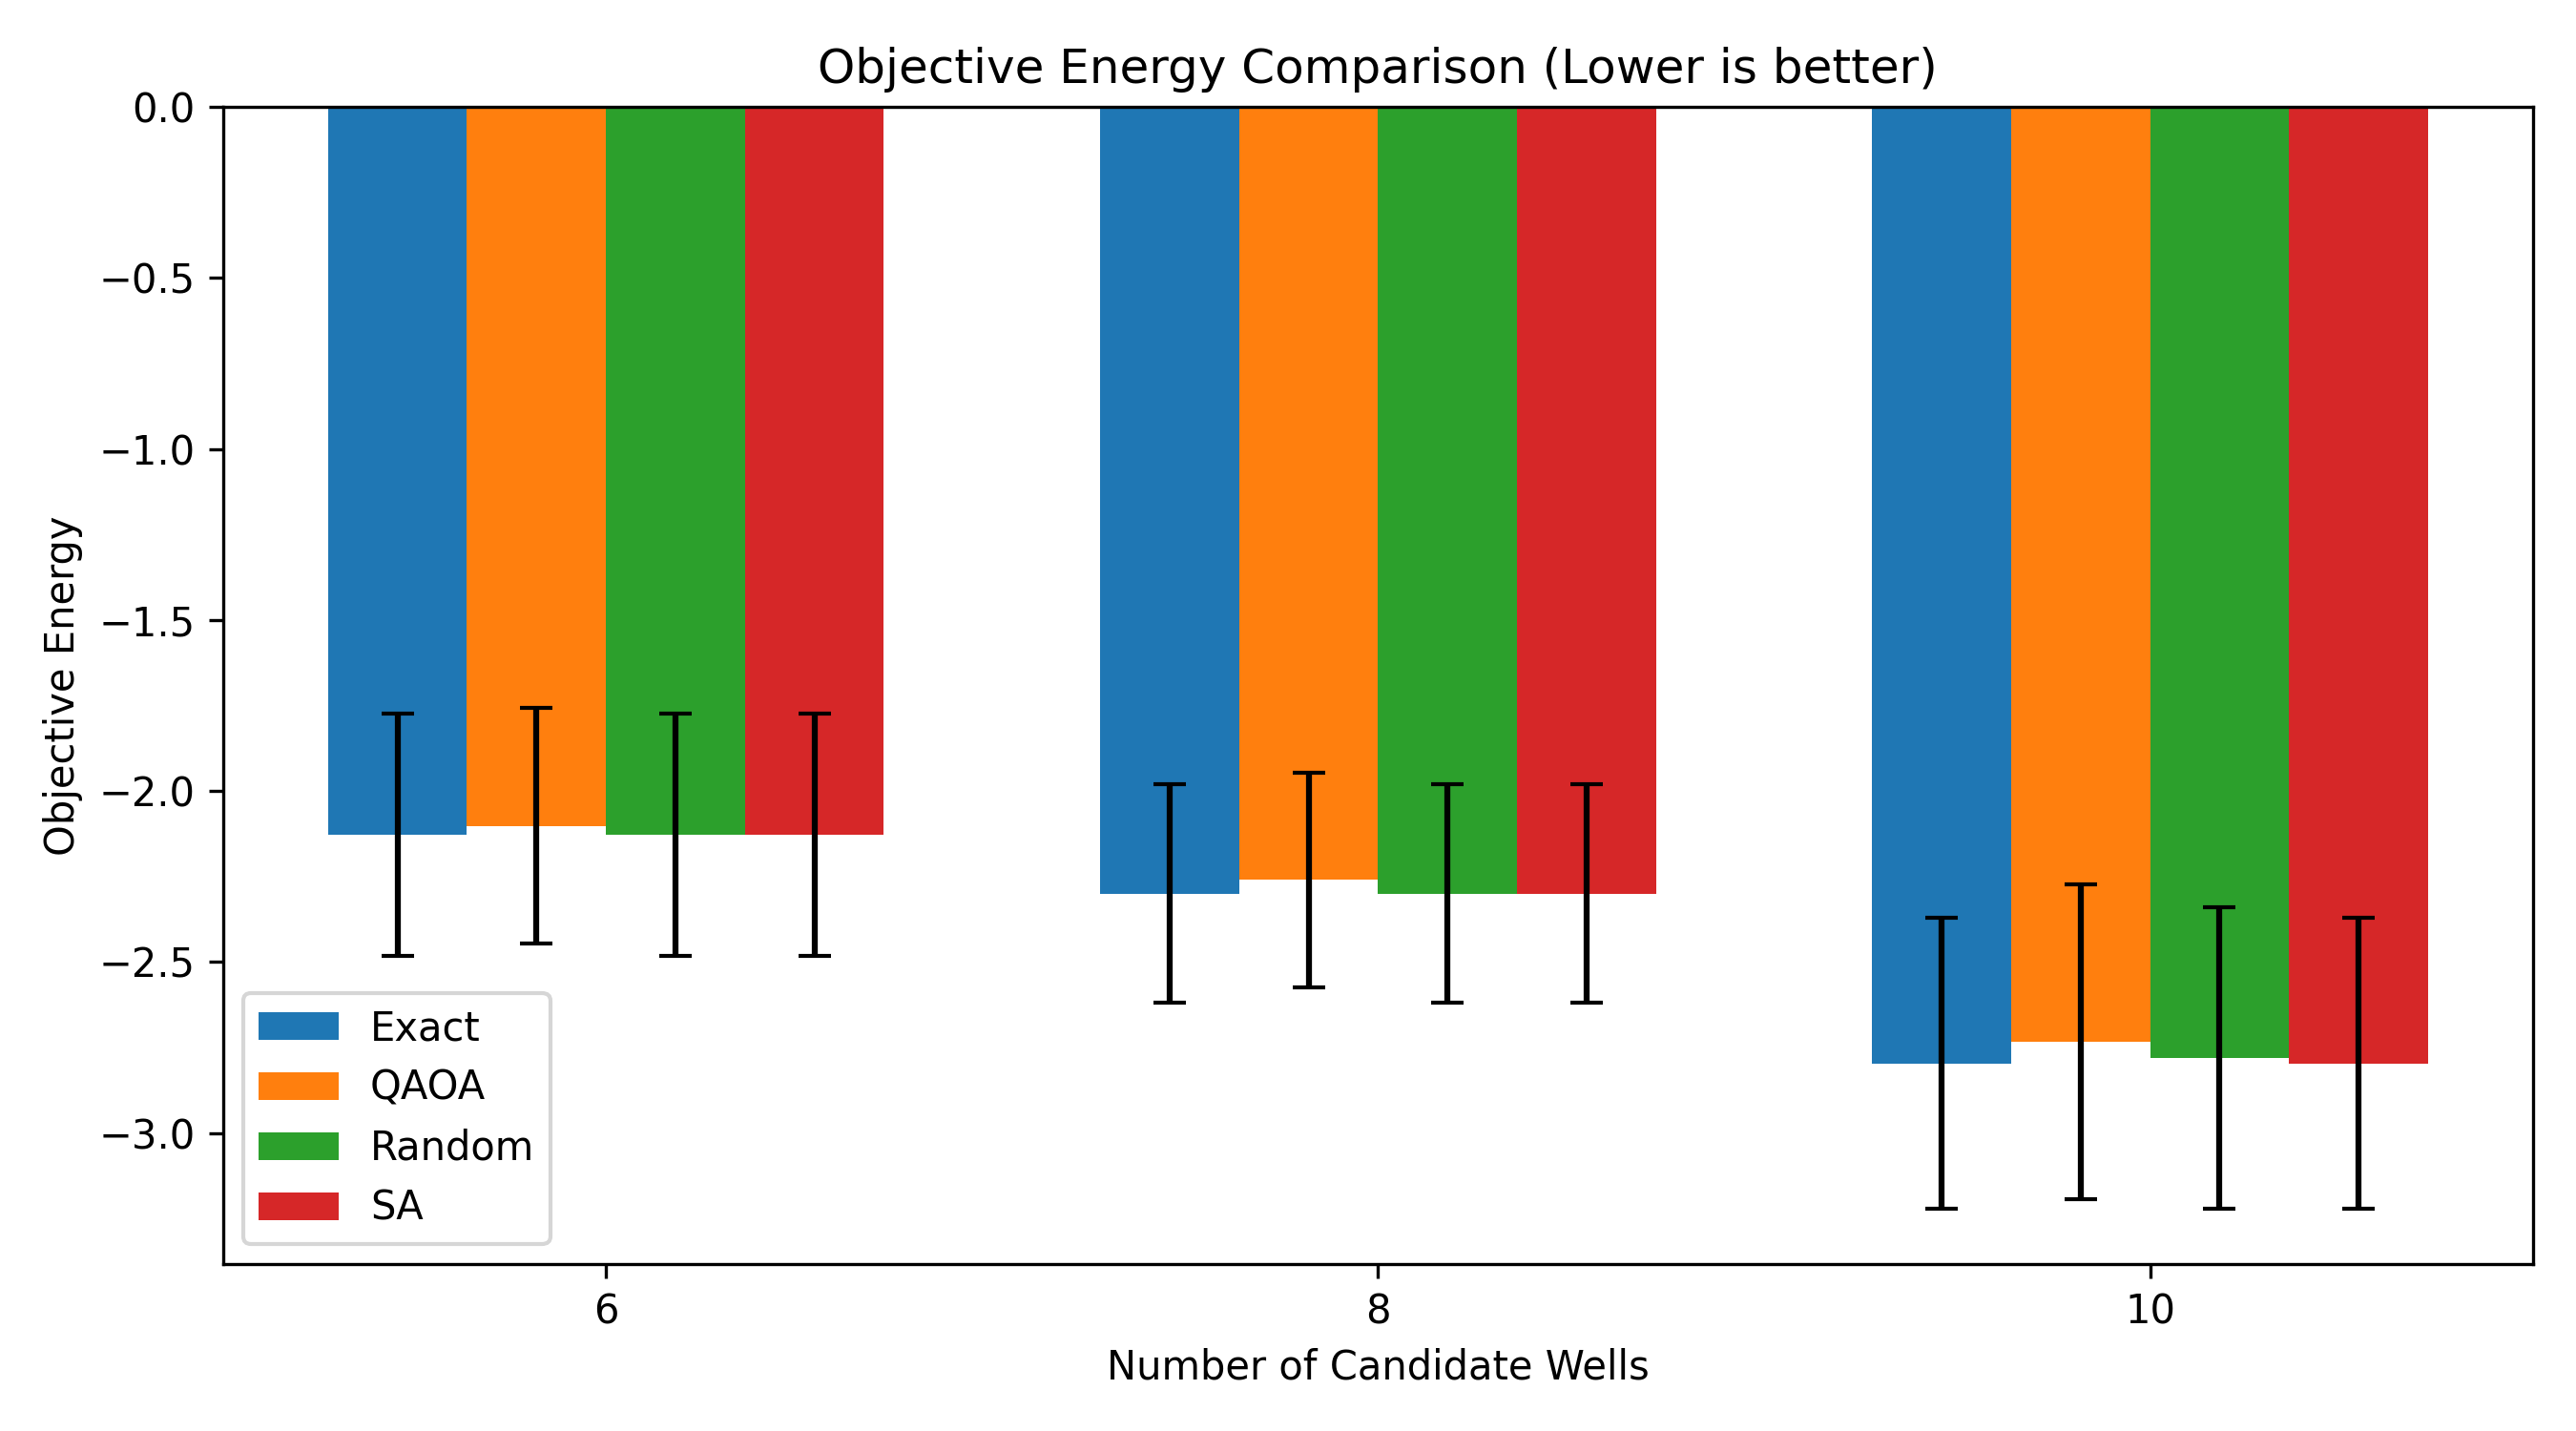
\includegraphics[width=0.78\textwidth]{energy_comparison.png}
\caption{Objective energy comparison. All three methods achieve the same optimal energy.}
\label{fig:energy}
\end{figure}

\begin{figure}[H]
\centering
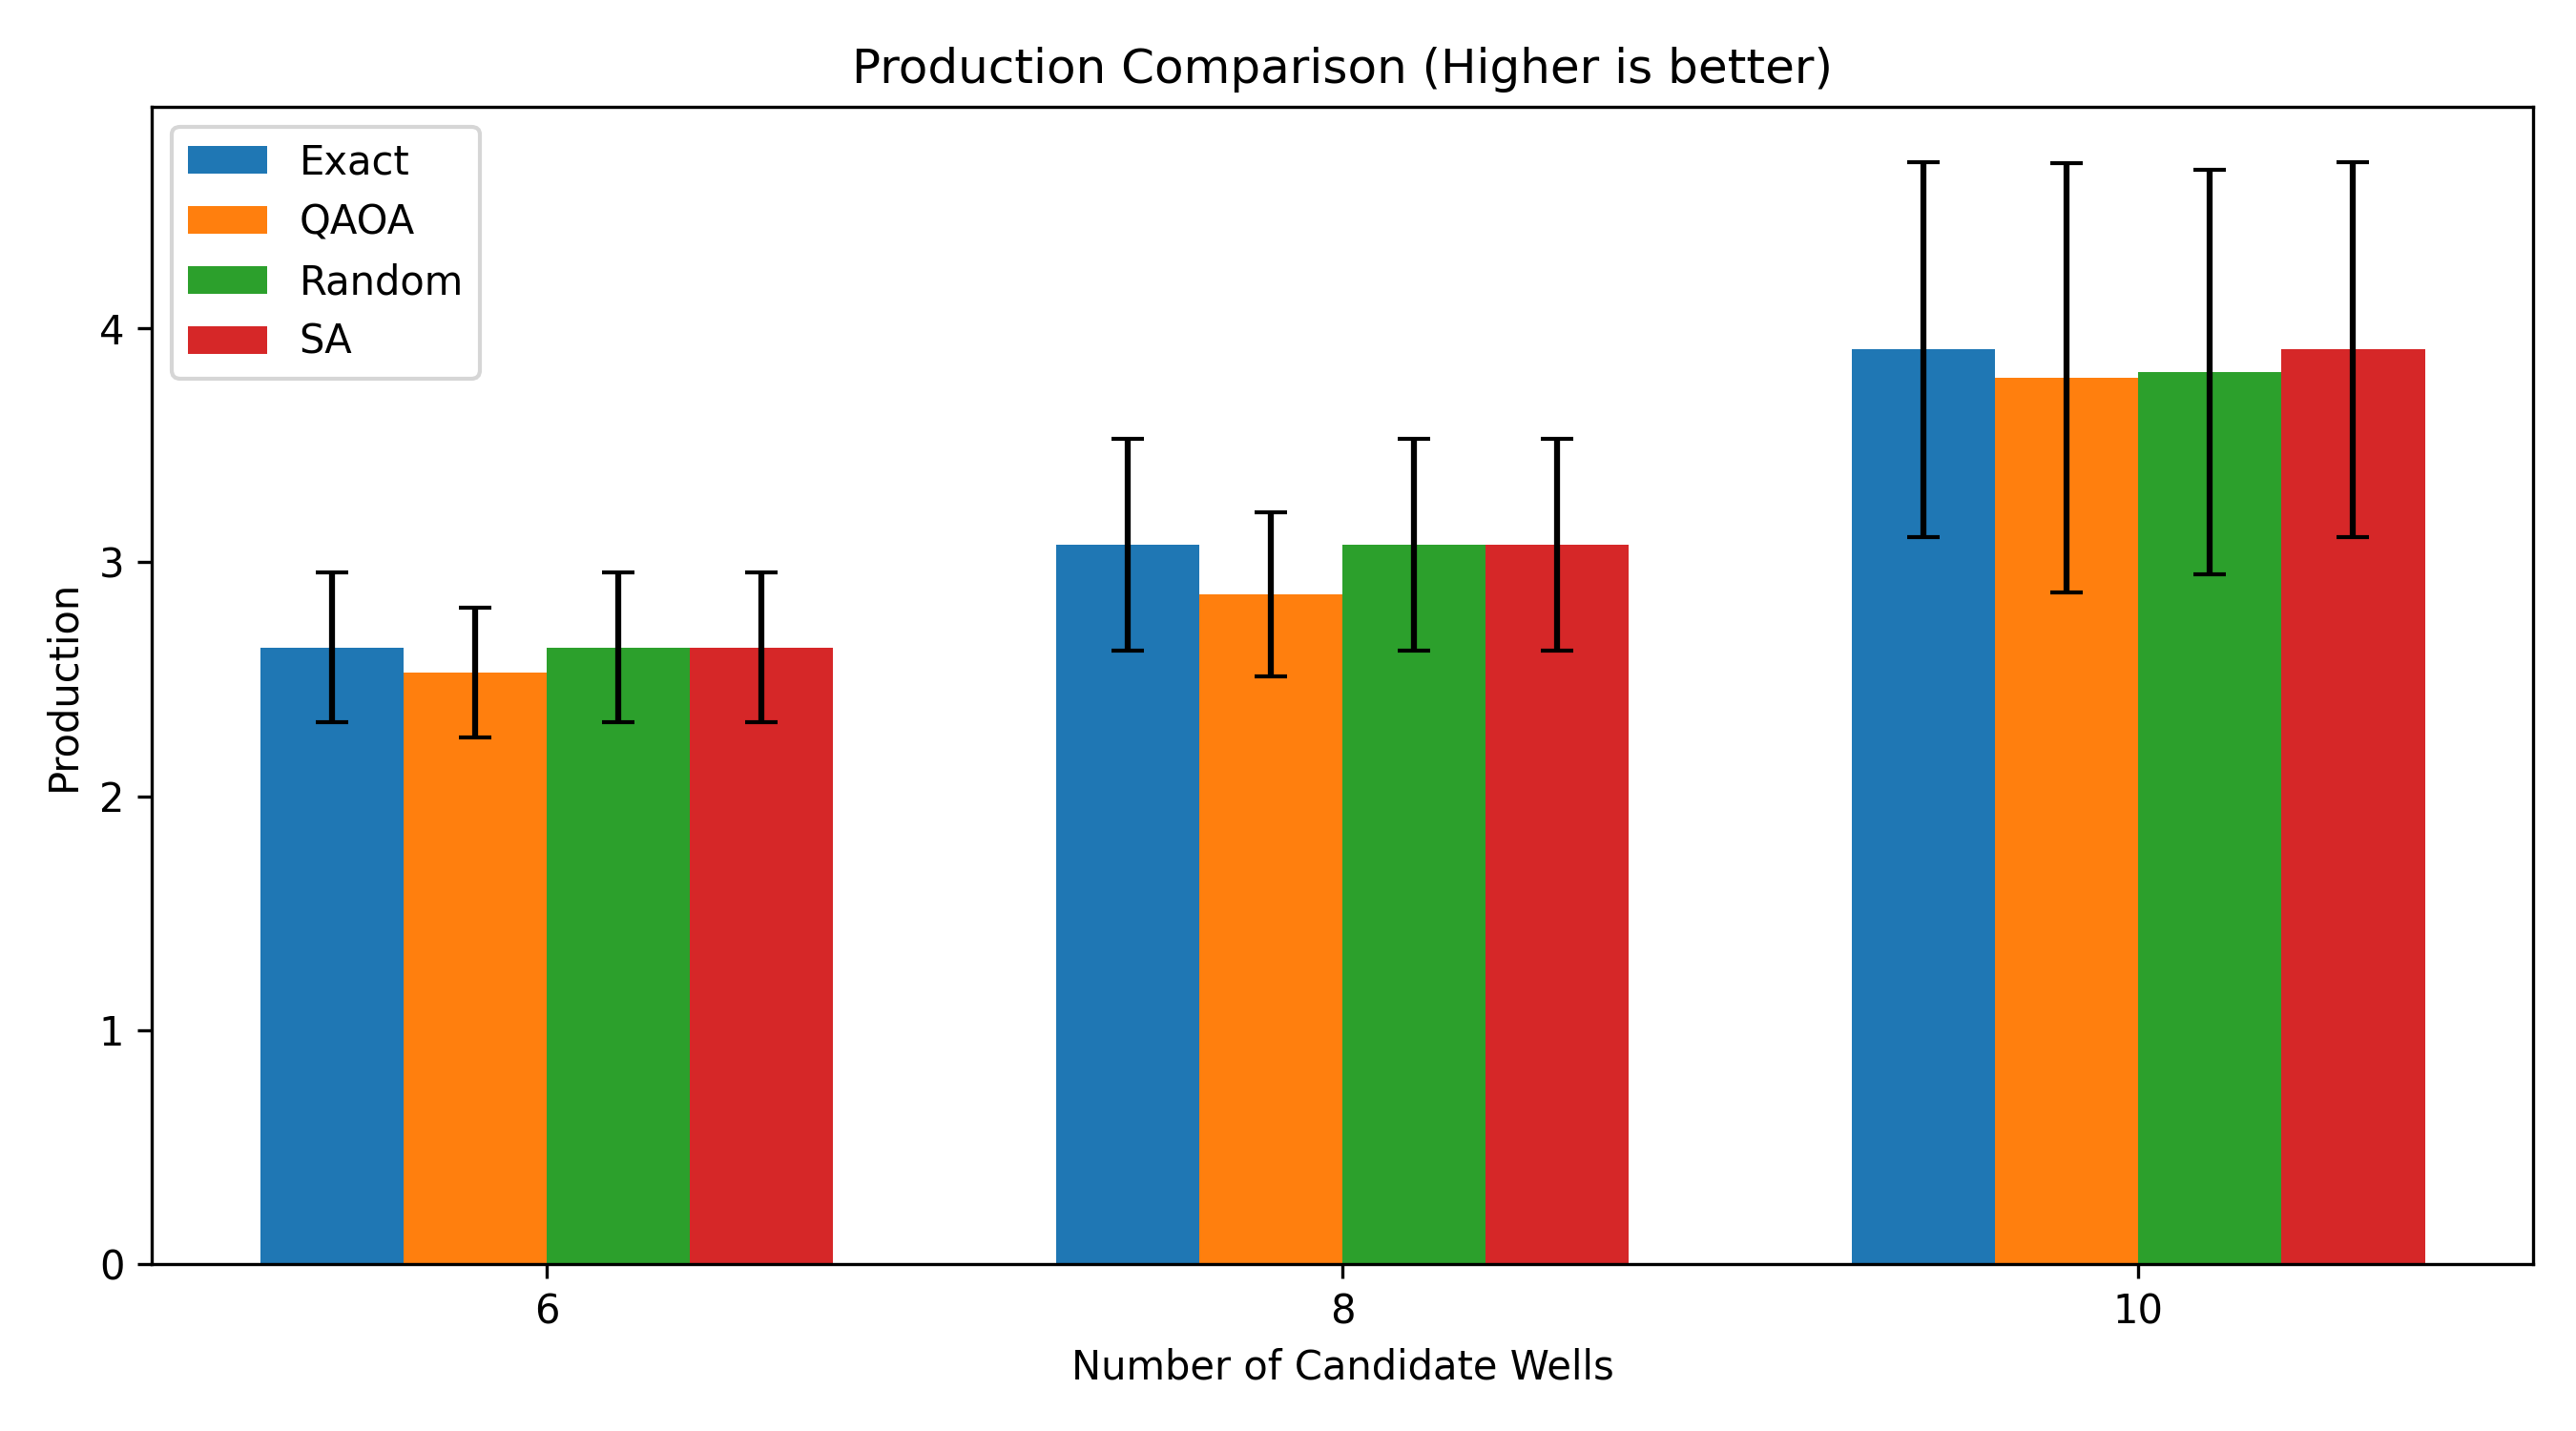
\includegraphics[width=0.78\textwidth]{production_comparison.png}
\caption{Total production of the selected well set.}
\label{fig:production}
\end{figure}

\begin{figure}[H]
\centering
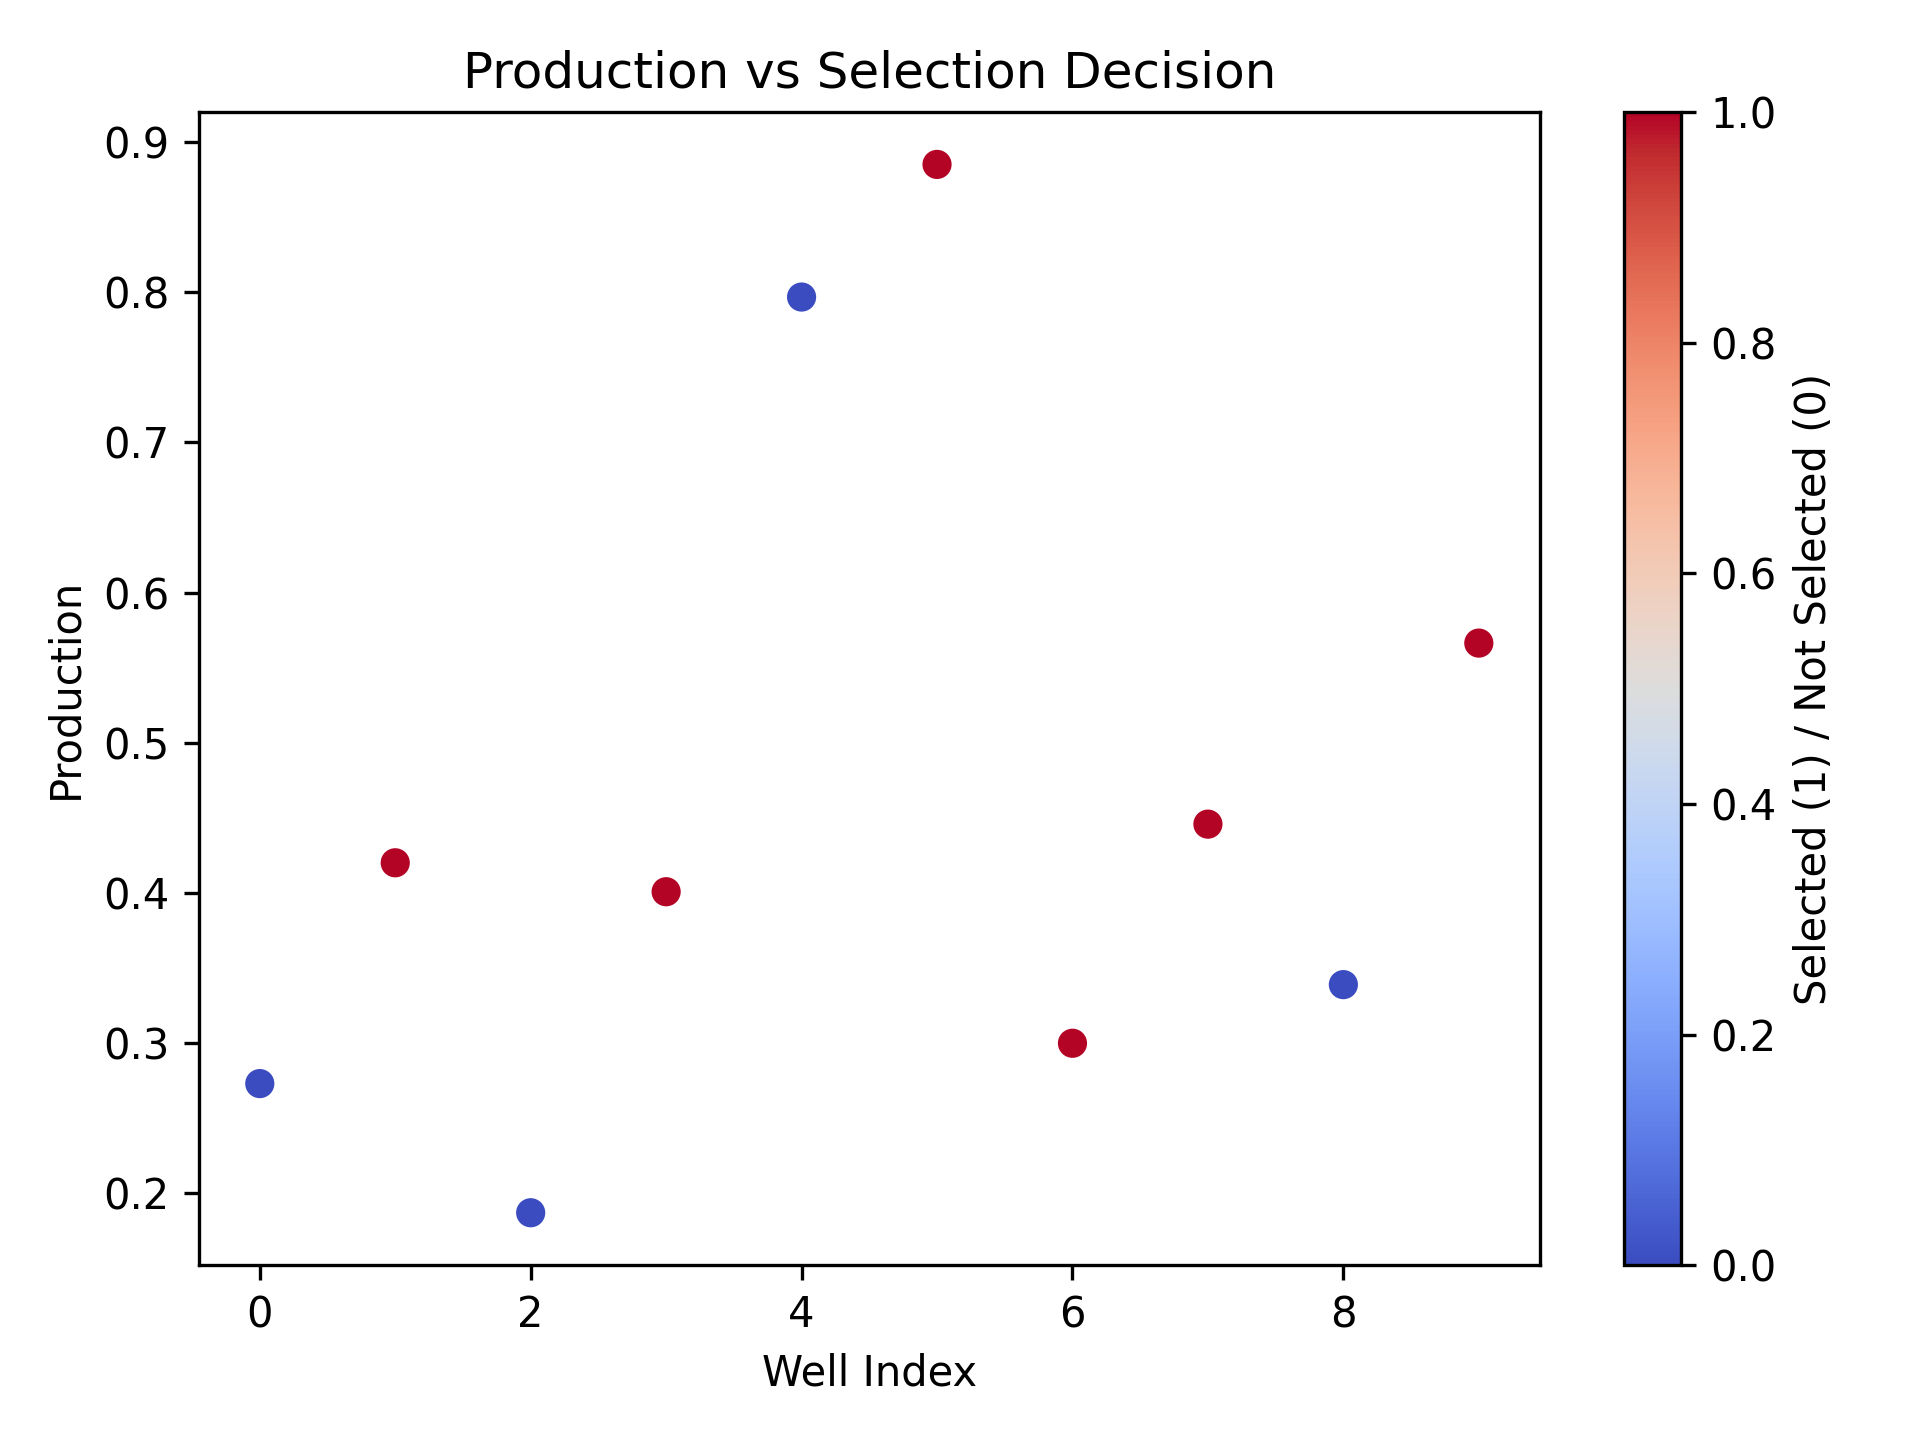
\includegraphics[width=0.78\textwidth]{production_scatter.png}
\caption{Production potential per well, with optimal selection highlighted in green.}
\label{fig:scatter}
\end{figure}

\begin{figure}[H]
\centering
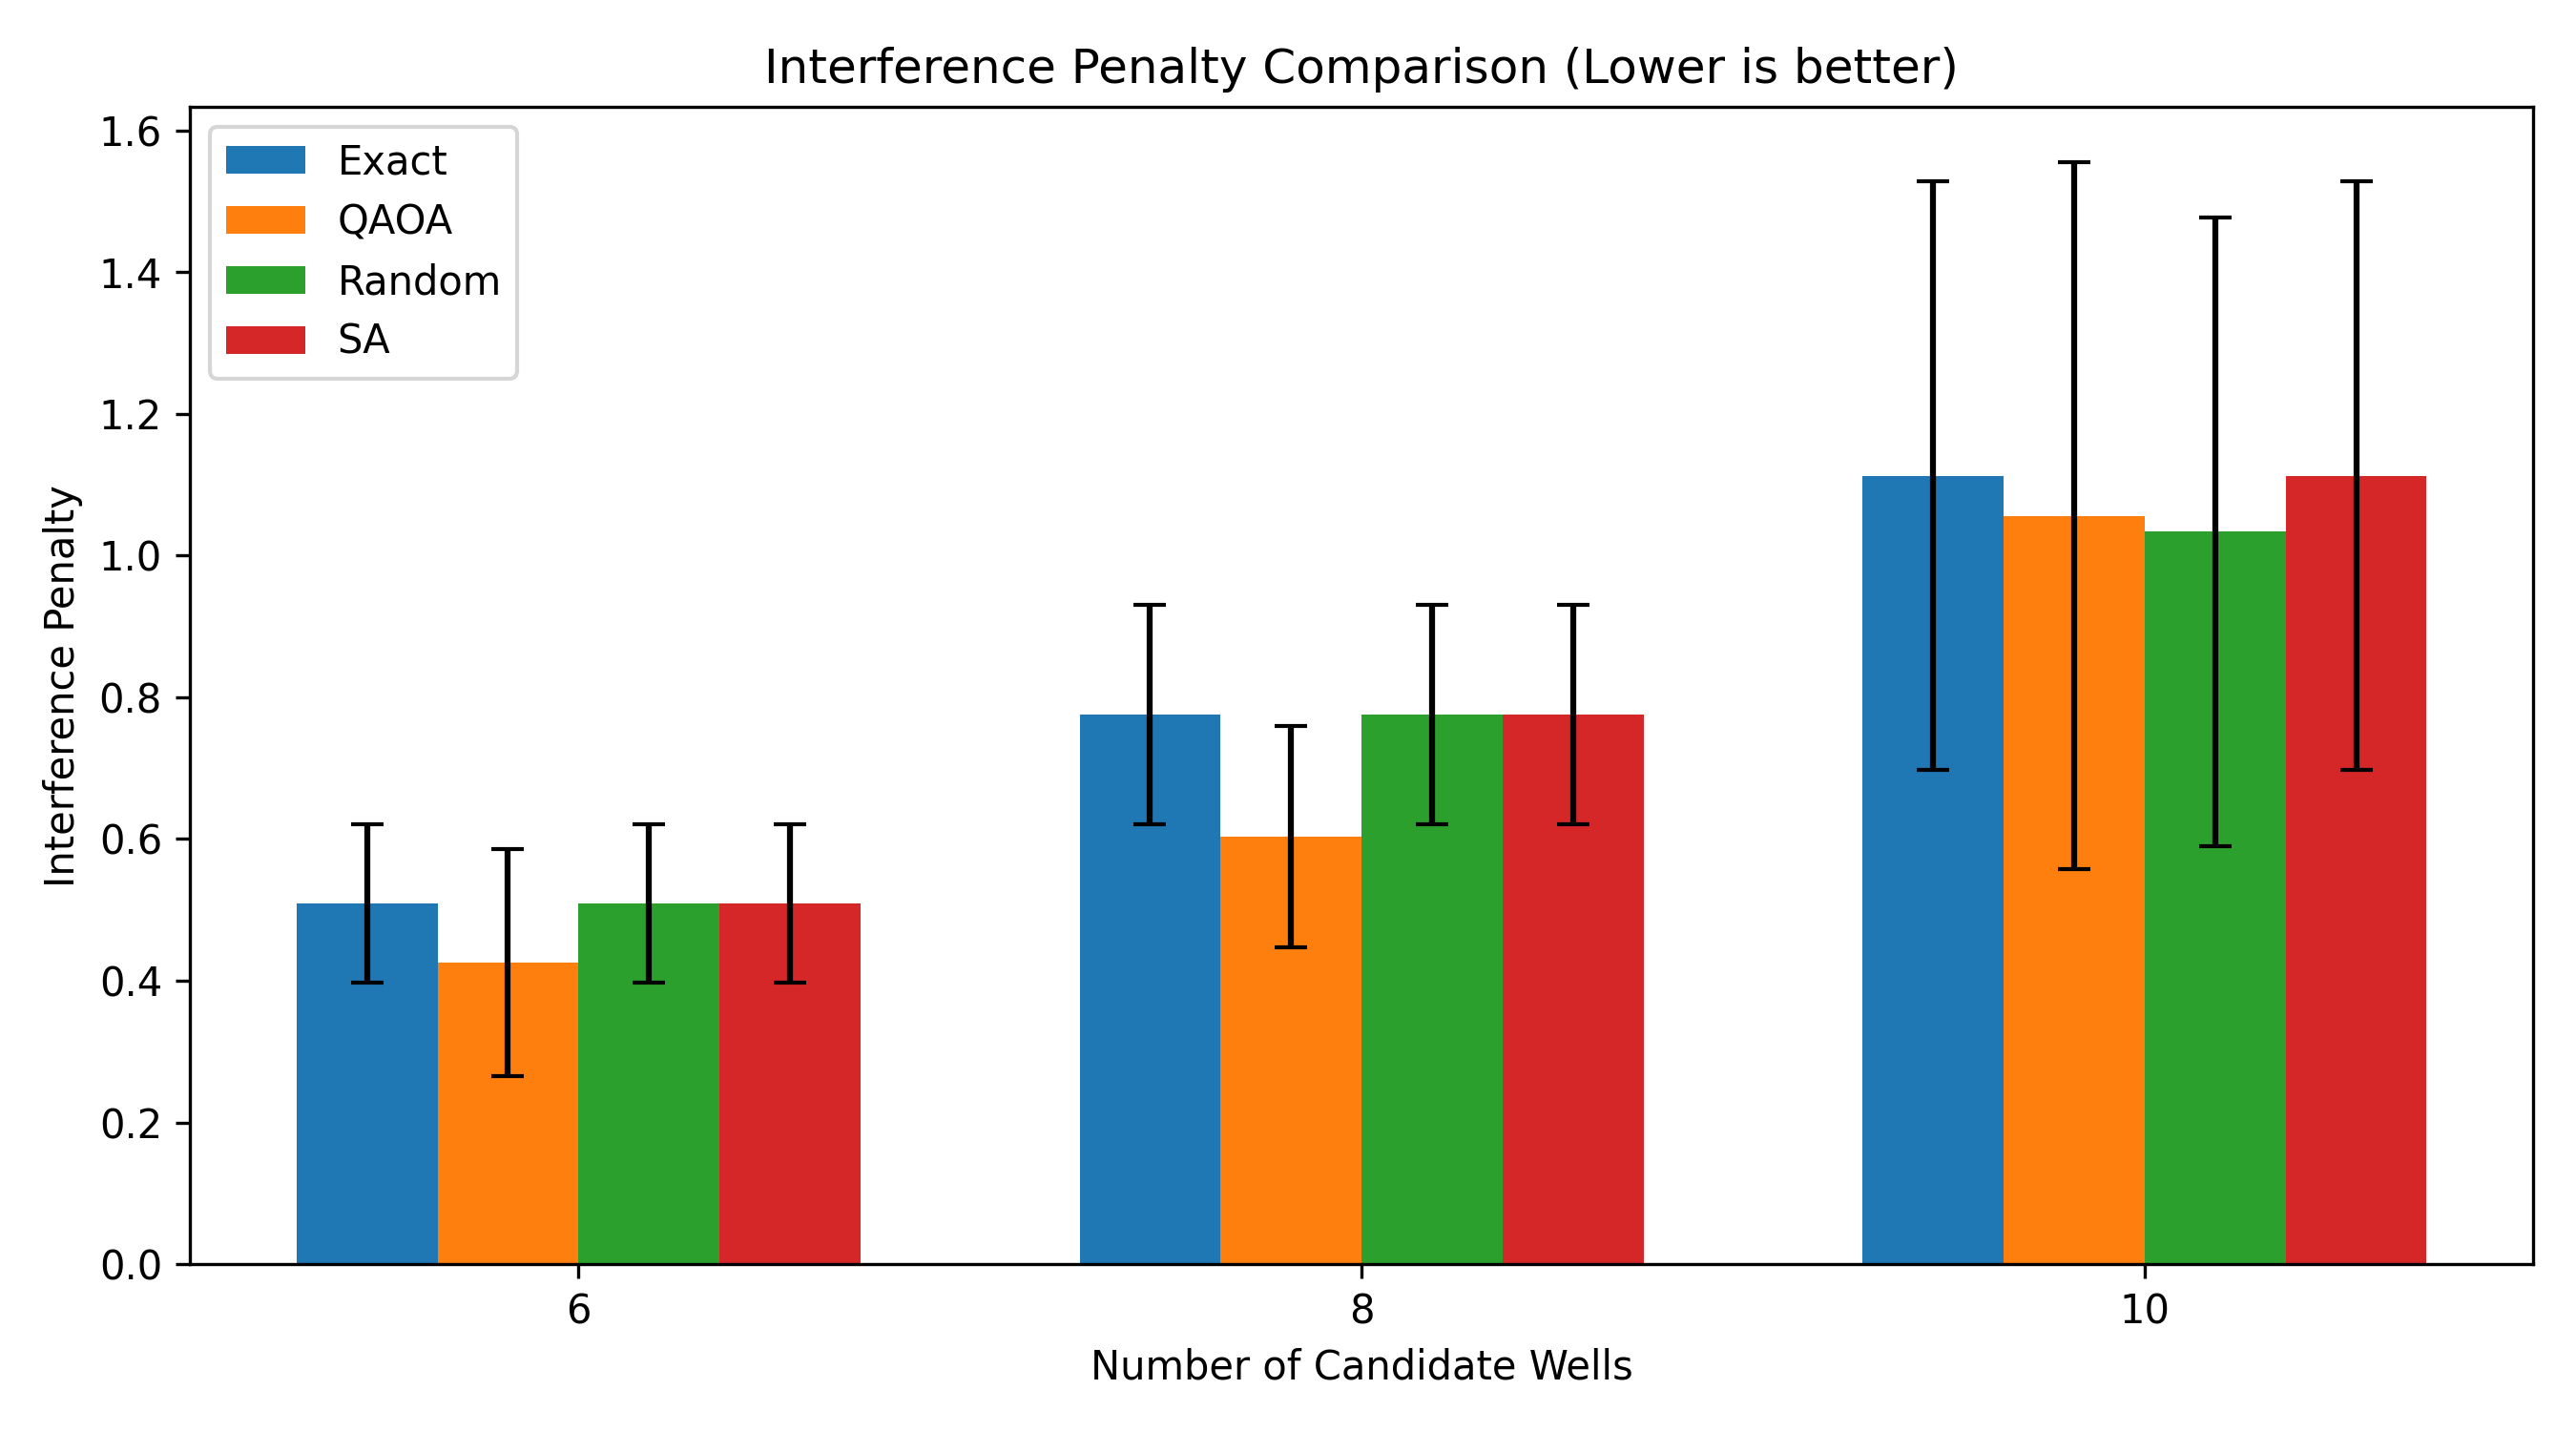
\includegraphics[width=0.78\textwidth]{interference_comparison.png}
\caption{Interference penalty for the selected configurations.}
\label{fig:interference}
\end{figure}

\begin{figure}[H]
\centering

\includegraphics[width=0.78\textwidth]{runtime_comparison.png}
\caption{Runtime comparison. QAOA simulation time is dominated by classical emulation overhead.}
\label{fig:runtime}
\end{figure}

\begin{figure}[H]
\centering

\includegraphics[width=0.78\textwidth]{results_plot.png}
\caption{Summary bar chart showing production potentials of all wells versus the selected subset.}
\label{fig:summary}
\end{figure}

\section{Discussion}

The updated implementation and this manuscript reflect a rigorous validation of the hybrid quantum--classical framework. Several key points deserve emphasis:

\paragraph{Correctness of the QUBO mapping.}
The construction \(Q_{ii} = -P_{i}\) and \(Q_{ij} = 0.2\exp(-d_{ij}/\lambda)\) is fully disclosed and reproducible. The Ising transformation given by Eqs.~\eqref{eq:ising_h} and~\eqref{eq:ising_J} is exact and allows direct implementation on gate-based quantum hardware.

\paragraph{Importance of solution extraction.}
The QAOA result is selected as the lowest-energy sampled bitstring, not the mode of the distribution. This aligns the evaluation metric with the objective function and avoids penalizing QAOA for dispersion in the output distribution. The fact that the optimal bitstring appears with modest frequency highlights the need for careful post-selection in variational quantum optimization.

\paragraph{Convergence gap and optimizer limitations.}
The expected QAOA energy during optimization (\(-1.482\)) remained above the optimal value (\(-1.702\)). This gap indicates that the variational state was not fully concentrated on the optimal solution, likely due to the limited depth \(p=2\) and the convergence behavior of COBYLA in a noisy, high-dimensional parameter landscape. Despite this, the presence of the optimal bitstring in the final distribution confirms that the parameterized circuit has the expressivity to capture the global minimum. Future work may explore alternative optimizers (e.g., SPSA, Bayesian optimization) or increased circuit depth to improve convergence.

\paragraph{Approximation ratio definition.}
The normalization using both \(E_{\text{best}}\) and \(E_{\text{worst}}\) provides a fair scale between 0 and 1. Because the worst energy is \(0.0\) for the all-zero state, the ratio simplifies to \(E_{\text{method}}/E_{\text{best}}\) in this specific instance.

\paragraph{Limitations of the benchmark.}
The four-well system is intentionally small to enable exact verification. It does not demonstrate quantum advantage, nor does it claim to. The purpose is to establish a baseline of correctness before scaling. In larger instances, the performance of QAOA may degrade unless circuit depth is increased appropriately, and the optimization landscape becomes more challenging. Additionally, the current study does not include specialized classical QUBO solvers (e.g., Gurobi, simulated bifurcation), which would provide a more complete performance baseline for future scaling studies.

\paragraph{Scalability considerations.}
While the results on \(N=4\) are encouraging, they do not guarantee similar performance on \(N=20\) or \(50\). The number of qubits required equals the number of candidate wells, and the number of two-qubit gates scales quadratically with \(N\) if all pairwise interactions are considered. On near-term quantum devices, noise and limited coherence times may significantly affect solution quality. Nevertheless, the validated framework provides a foundation for investigating quantum-inspired heuristics in larger reservoir development scenarios.

\section{Conclusion}

The hybrid quantum--classical framework successfully solves the well placement problem on a fully verifiable four-well benchmark. The QUBO formulation captures the trade-off between production and interference, and the QAOA implementation (with proper solution extraction) recovers the exact global optimum. This work provides a validated foundation for extending the methodology to larger candidate sets and more complex reservoir models.

\section*{Author Contributions}
Tareq Mageed conceived the study, developed the optimization framework, implemented the computational workflow, performed the analysis, and wrote the manuscript.

\section*{Conflict of Interest}
The author declares no conflict of interest.

\section*{Data Availability}
The complete Python code and results are included in the supplementary materials and the \texttt{results/} directory.

% ==========================================================
% المراجع (References)
% ==========================================================
\begin{thebibliography}{9}

\bibitem{farhi2014quantum}
E. Farhi, J. Goldstone, and S. Gutmann, ``A quantum approximate optimization algorithm,'' arXiv preprint arXiv:1411.4028, 2014.

\bibitem{virtanen2020scipy}
P. Virtanen et al., ``SciPy 1.0: fundamental algorithms for scientific computing in Python,'' \textit{Nature Methods}, vol. 17, pp. 261--272, 2020.

\bibitem{qiskit2024}
Qiskit contributors, ``Qiskit: An open-source framework for quantum computing,'' 2024. [Online]. Available: \url{https://qiskit.org}

\bibitem{powell1994direct}
M. J. D. Powell, ``A direct search optimization method that models the objective and constraint functions by linear interpolation,'' in \textit{Advances in Optimization and Numerical Analysis}, Springer, 1994, pp. 51--67.

\end{thebibliography}

\end{document}
